%%%%%%%%%%%%%%%%%%%%%%% file typeinst.tex %%%%%%%%%%%%%%%%%%%%%%%%%
%
% This is the LaTeX source for the instructions to authors using
% the LaTeX document class 'llncs.cls' for contributions to
% the Lecture Notes in Computer Sciences series.
% http://www.springer.com/lncs       Springer Heidelberg 2006/05/04
%
% It may be used as a template for your own input - copy it
% to a new file with a new name and use it as the basis
% for your article.
%
% NB: the document class 'llncs' has its own and detailed documentation, see
% ftp://ftp.springer.de/data/pubftp/pub/tex/latex/llncs/latex2e/llncsdoc.pdf
%
%%%%%%%%%%%%%%%%%%%%%%%%%%%%%%%%%%%%%%%%%%%%%%%%%%%%%%%%%%%%%%%%%%%


\documentclass[runningheads,a4paper]{llncs}

\usepackage{amssymb}
\setcounter{tocdepth}{3}
\usepackage{graphicx}
\usepackage{url}
%\usepackage{url}
%\urldef{\mailsa}\path|{sbendoukha, .haas, frank.holzwarth,|
%\urldef{\mailsb}\path|anna.kramer, leonie.kunz, christine.reiss, nicole.sator,|
%\urldef{\mailsc}\path|erika.siebert-cole, peter.strasser, lncs}@springer.com|    
\newcommand{\keywords}[1]{\par\addvspace\baselineskip
\noindent\keywordname\enspace\ignorespaces#1}
%% ------------------------------------------------------------------- %%
%%  File:     newcommand.tex                                           %%
%%  Encoding: Latin-1 = ISO 8859-1                                     %%
%%  Author:   TGI et al                                                %%
%%  Created:  long ago                                                 %%
%%  Updated:  15.01.2010                                               %%
%%  Updated:  Here we should use the feature of automatic update,      %%
%% 	          as we use it in the Herold project.                      %%
%%                                                                     %%
%% ------------------------------------------------------------------- %%
%FUER Handout:
\newcommand{\remarks}[1]{{\bf~Remarks~???:}{\em\small #1}\\{\bf~Remarks end}}
%NICHT Fuer Handout:
%\newcommand{\remarks}[1]{}
\newcommand{\RenewGrass}{\textsc{RenewGrass}}
\newcommand{\fig}{Figure}
\newcommand{\Fig}{Figure}
\newcommand{\figs}{Figures}
\newcommand{\Figs}{Figures}
\newcommand{\sect}{Section}
\newcommand{\Sect}{Section}
\newcommand{\code}[1]{\texttt{#1}}
\newcommand{\Renew}{\textsc{Renew}}
\newcommand{\renew}{\Renew{}}
\newcommand{\Sam}{\textsc{Sam}}
\newcommand{\Mrt}{\textsc{Mrt}}
\newcommand{\Agnes}{{\textsc{Agnes}}}
\newcommand{\Mulan}{\textsc{Mulan}}
\newcommand{\Paose}{\textsc{Paose}}
\newcommand{\Paosel}{\textsc{Petri net-based, Agent-Oriented Software Engineering}}
\newcommand{\Sonar}{\textsc{Sonar}}
\newcommand{\Nin}{Nets-within-nets}
\newcommand{\nin}{nets-within-nets}
\newcommand{\nc}{net component}
\newcommand{\Nc}{Net component}
\newcommand{\NC}{Net Component}
\newcommand{\ncs}{net components}
\newcommand{\Ncs}{Net components}
\newcommand{\NCs}{Net Components}
\newcommand{\cpn}{colored Petri net}
\newcommand{\cpns}{colored Petri nets}
\newcommand{\NIN}{Nets-Within-Nets}
\newcommand{\Pn}{Petri~net}
\newcommand{\Pns}{Petri~nets}
\newcommand{\Capa}{\textsc{Capa}}
\newcommand{\Ace}{\textsc{Ace}}
\newcommand{\referencenets}{reference nets}
\newcommand{\Referencenets}{Reference nets}
\newcommand{\referencenet}{reference net}
\newcommand{\Referencenet}{Reference net}
\newcommand{\rn}{\referencenet{}}
\newcommand{\Rn}{\Referencenet{}}
\newcommand{\rns}{\referencenets{}}
\newcommand{\Rns}{\Referencenets{}}
\newcommand{\downlink}{downlink}
\newcommand{\Downlink}{Downlink}
\newcommand{\uplink}{uplink}
\newcommand{\Uplink}{Uplink}
\newcommand{\longpage}{\enlargethispage{\baselineskip}}
\newcommand{\Longpage}{\enlargethispage{2\baselineskip}}
\newcommand{\todo}[1] {{\bf TODO:\ \small \texttt{#1}}\marginpar{todo}}
\newcommand{\opinion}[1]{{\bf {\sc Opinion}:\ \small \texttt{#1}}\marginpar{Opinion}}
\newcommand{\Java}{\textsl{Java}}
\newcommand{\Fipa}{{\sc Fipa}}
\newcommand{\Jade}{{\sc Jade}}

\newcommand{\aip}{agent interaction protocol diagram}
\newcommand{\aips}{agent interaction protocol diagrams}
\newcommand{\Aip}{Agent interaction protocol diagram}
\newcommand{\Aips}{Agent interaction protocol diagrams}
\newcommand{\AIPs}{Agent Interaction Protocol Diagrams}
\newcommand{\AIP}{Agent Interaction Protocol Diagram}
\newcommand{\Mup}{protocol net}
\newcommand{\Mups}{protocol nets}
\newcommand{\MUP}{Protocol net}
\newcommand{\MUPS}{Protocol netss}

\newcommand{\mas}{multi-agent system}
\newcommand{\mass}{multi-agent systems}
\newcommand{\Mas}{Multi-agent system}
\newcommand{\Mass}{Multi-agent systems}
\newcommand{\MAS}{Multi-Agent System}
\newcommand{\MASS }{Multi-Agent Systems}

\newcommand{\maa}{multi-agent application}
\newcommand{\maas}{multi-agent applications}
\newcommand{\Maa}{Multi-agent application}
\newcommand{\Maas}{Multi-agent applications}
\newcommand{\MAA}{Multi-Agent Application}
\newcommand{\MAAS }{Multi-Agent Applications}

\newcommand{\mm}[1]{~}
\newcommand{\ooed}{ob\-ject-orien\-ted}
\newcommand{\ins}[1]{\code{#1}}
\newcommand{\emp}[1]{\emph{#1}}

    \newtheorem{defi}{Definition}
    \newtheorem{unterdefi}{}[defi]


\newcommand{\plin}{plug-in}
\newcommand{\Plin}{Plug-in}
\newcommand{\plinsys}{plug-in system}
\newcommand{\source}[1]{\code{#1}}
\newcommand{\eclipse}[0]{\emph{eclipse}}
%\newcommand{\mode}[0]{\emph{Mode}}
\newcommand{\net}[0]{\emph{.NET}}
\newcommand{\sofa}[0]{\emph{SOFA}}
\newcommand{\package}[1]{\textsl{package} \source{#1}}
\newcommand{\pack}[0]{\textsl{package}}
\newcommand{\packages}[0]{\textsl{package}s}
\newcommand{\file}[1]{\textbf{#1}}
\newcommand{\komp}[1]{\textbf{#1}}

\newcommand{\name}[1]{\textsc{#1}}

\newcommand{\englisch}[1]{#1}
\newcommand{\ep}[0]{\englisch{Extension Point}}

\newcommand{\plname}[1]{#1}

\newcommand{\UoH}{University of Hamburg}


\renewcommand{\topfraction}{0.9}

%%% Local Variables: 
%%% mode: latex
%%% TeX-master: "workfl-agents"
%%% End: 

\begin{document}

\mainmatter  % start of an individual contribution

% first the title is needed
\title{On the Use of Reference Nets for Building Cloud-based Scientific Workflows}

% a short form should be given in case it is too long for the running head
\titlerunning{Cloud-based Image Processing}

% the name(s) of the author(s) follow(s) next
%
% NB: Chinese authors should write their first names(s) in front of
% their surnames. This ensures that the names appear correctly in
% the running heads and the author index.
%
\author{Hayat Bendoukha\inst{1}%
%\thanks{Please note that the LNCS Editorial assumes that all authors have used
%the western naming convention, with given names preceding surnames. This determines
%the structure of the names in the running heads and the author index.}%
\and Sofiane Bendoukha\inst{2}\and Yahya Slimani \inst{3}}
%
\authorrunning{Hayat Bendoukha et al.}
% (feature abused for this document to repeat the title also on left hand pages)

% the affiliations are given next; don't give your e-mail address
% unless you accept that it will be published
\institute{Department of Computer Science\\
Faculty of Mathematics and Computer Science\\
Université des Sciences et de la Technologie d'Oran Mohamed Boudiaf, USTO-MB, BP 1505, El M'naouer,  31000  Oran Algérie\\
\texttt{bendoukhayat@univ-usto.dz}
\and
Theoretical Foundations of Computer Science (TGI)\\
Department of Informatics, University of Hamburg, Germany\\
\texttt{sbendoukha@informatik.uni-hamburg.de}\\
\and
Département Informatique
Institut Supérieur des Arts Multimédia (ISAMM)
Université de la Manouba
 \\
Campus Universitaire, 2010 Manouba, Tunisie\\
\texttt{yahya.slimani@fst.rnu.tn}
}
 
%
% NB: a more complex sample for affiliations and the mapping to the
% corresponding authors can be found in the file "llncs.dem"
% (search for the string "\mainmatter" where a contribution starts).
% "llncs.dem" accompanies the document class "llncs.cls".
%

\toctitle{Lecture Notes in Computer Science}
\tocauthor{Sofiane Bendoukha, Hayat Bendoukha, Daniel Moldt}
\maketitle


\begin{abstract}
Cloud computing provides scientists with a large number of powerful resources.
%
These resources enhance the productivity of the whole system.
%
Running complex scientific workflows on Cloud resources rather then on-premise increases the performance of execution.
%
Nevertheless, traditional scientific workflow management (SWfM) systems are not yet adapted for the Cloud.
%
Creation of scientific workflows and their execution in the Cloud still face many challenges due to the complexity of the Cloud environment. 
%
Migrating a part or the whole scientific application to the Cloud is not trivial .
%
It should be based on a solid strategy.
%
Questions like: Where to store the data and where to execute the processes need to be investigated.
%
In this paper, we first present \RenewGrass{}, a tool for modeling and executing image processing workflows by \emph{reference nets}.
%
Then, we discuss the deployment of \RenewGrass{} into the Cloud.
%
This work includes also a use case example related to the remote sensing domain.
%
%Here we should emphasize the results provided in this paper.


\keywords{Workflows, \RenewGrass, Petri Nets, Cloud computing, Image processing}
\end{abstract}


\section{Introduction}
%!TEX root = ./FMi_2015_AISC.tex
%
% UTF8-Check: Umlaute: äöüÄÖÜß
%
\label{sec:introduction}
%
\emph{Scientific workflows} are a special class of workflows, which are characterized as large-scale, long-running and resource-intensive  \cite{scientific}. 
%Different domains can benefit from the Cloud. 
%
The major goal of scientific workflows is to allow scientists to focus on domain-specific (science) aspects of their work, rather than dealing with complex data management and software issues. 
%In the current work, we focus on \emph{scientific workflows}, which are characterized as large-scale and long-running.
%
How the sequence of the workflow tasks is represented can be handled in different ways.
%
The sequence can be specified either by scripting languages or through graph-based techniques such as Petri nets or $ \pi $-calculus \cite{Aalst03picalculus} \cite{smith04pi}.
%
Scripting languages are usually based on markup languages such as
Extensible Markup Language (XML). They may be convenient for well skilled users and do not need to be converted to be run on a cloud environment. But, they are not user-oriented and do not permit to  specify large and complex workflows manually \cite{hayatndt}. 
%
In this work, Petri nets and more specifically \textit{reference nets} \cite{Kummer02} as a modeling technique suitable to model the workflow patterns
in an elegant and easy way \cite{sofiane}.

Nevertheless, due to the large amount of data and tasks, that need to be processed, the execution of such kind of workflows requires often to be mapped into external resources.
%
During these a few years, Cloud computing is growing considerably and it is gaining popularity in both academia and industry.
%
We believe that this technology is the suitable solution for the execution of scientific workflows.
%
The reason is the  features that clouds  provide in terms of the powerful resources, which range from storage, computing and networks.
%
Unfortunately, existing SWfM systems are not adapted to perform in the Cloud.
%
They need to fit to the Cloud architecture.
%
They also need to provide modeling means and migration mechanisms that enable a full integration between workflow concepts and Cloud technology.


The objective of the current work is twofold.
%
First, we implemented a tool named \RenewGrass{} for the specification and the execution of scientific workflows.
%
Then, we, successfully, integrated \RenewGrass{} in the \textbf{RE}ference \textbf{NE}ts \textbf{W}orkshop (\Renew{}) which is available at (\url{www.renew.de}), our chosen modeling and simulation tool for Petri nets.
%
%\RenewGrass{} has been successfully integrated in the \textbf{RE}ference \textbf{NE}ts \textbf{W}orkshop (\Renew{}) which is available at (\url{www.renew.de}), our chosen modeling and simulation tool for Petri nets.
%
As a domain of application, the tool is suitable for remote sensing especially processing of satellite imagery.
%
% \cite{Diverse Papiere zu RenewGrass!}
%
Modeling and implementing such kind of workflows need specific tools and techniques, which are unfortunately not provided by \Renew{}.
%
Technically, the integration of \RenewGrass{} consists on extending  \Renew{} by modules and components of the Geographic Resource Analysis Support System (\textsc{Grass}) GIS (Geographic Information System).
%Technically, the Geographic Resource Analysis Support System (\textsc{Grass}) GIS (Geographic Information System) modules \cite{GRASS_GIS_software} have been successfully integrated with \Renew{}. 
%
This allows users to invoke Grass GIS modules directly from their Petri net models, which can be later executed.
%
With the integration of \RenewGrass{} into \Renew{}, the latter is now able to deal with other research domains such as the scientific domain.
%
Moreover, as soon as the workflow requirements become locally unsatisfied, workflow tasks need to be mapped to distributed resources.
%
With respect to the work presented in \cite{Bendoukha+15c} and as an extension, this issue is also taken into account, since our long-term perspective is to provide a service-oriented environment built on top of Cloud resources and to allow flexible deployment of scientific workflows.
%
Therefore, we will discuss the deployment of \RenewGrass{} into the Cloud.
%
Questions like: Where to store the data? Where to execute the activities? will be investigated.
%
Here, we propose an agent-based architecture, where each functionality of the system is performed by a specific agent.
%
In our approach, we follow the \Paosel{} (\Paose{}) paradigm for developing agent-based applications.
%

%%Remainder of the paper
The rest of the paper is organized as follows. 
%
Related work as well as the conceptual and technical background of this work are presented in Section.~\ref{sec:functionality}.
%
\RenewGrass{} is described in Section.~\ref{sec:grassintegration}. 
%
How \RenewGrass{} can be deployed in the Cloud is investigated in Section.~\ref{sec:Cloudmigration}.
%
%The drawbacks of the current implementations and propose further solutions are discussed in Section.~\ref{sec:discussion}.
Section.~\ref{sec:discussion} discusses .
%
Section.~\ref{sec:conclusion} concludes the paper with summary and future works.







\section{Related Work and Background}
\label{sec:functionality}
%
It is noteworthy to introduce some concepts, techniques and tools that constitute the conceptual and functional background of this work.
%
These are essential to understand how the contributions work.

%Before going further in the presentation of \RenewGrass{} it is necessary to introduce some concepts, techniques and tools that constitute the conceptual and functional background of this work.
%
\subsection{Cloud Computing}
%
Cloud computing is a model for enabling ubiquitous, convenient, on-demand network access to a shared pool of configurable computing resources (e.g., networks, servers, storage, applications, and services).
%
Cloud computing can be viewed as a collection of services, which can be presented as a set of loosely-coupled layers \cite{Mell+11}.
%
These service models are closely related and can be seen as three layers, which are the Infrastructure as a Service (IaaS), the Software as a Service (SaaS) and the Platform as a Service (PaaS).
%
Before the emergence of the Cloud technology, there were significant research projects dealing with the development of distributed and scientific workflow systems with the grid paradigm. 
%
Workflow enactment service can be built on top of the low level grid middle-ware (eg. Globus Toolkit\footnote{http://www.globus.org/toolkit/}, UNICORE\footnote{http://www.unicore.eu/}, EGI \footnote{https://www.egi.eu/} and Alchemi\footnote{http://www.cloudbus.org/$ \sim $alchemi/}), through which the workflow management system invokes services provided by grid resources \cite{YuB05}.
%
At both the build-time and run-time phases, the state of the resources and applications can be retrieved from grid information services. 
%
There are many grid workflow management systems in use; like these representative projects: ASKALON \footnote{\url{http://www.askalon.org/}}, Pegasus \footnote{\url{http://www.pegasus.org/}}, Taverna \footnote{\url{http://www.taverna.org.uk/}}, Kepler\footnote{\url{https://kepler-project.org/}}, Triana\footnote{\url{http://www.trianacode.org/}} and Swift \cite{Zhao+11}.
%
Most of these projects, have been investigating the adaptation of their architectures to include the Cloud technology.
%
For instance, the Elastic Compute Cloud (EC2) module has been implemented to make Kepler supports Amazon Cloud services.
%
Launched in 2012, the Amazon Simple Workflow (SWF)\footnote{aws.amazon.com/swf} is an orchestration service for building scalable applications.
%
It maintains the execution state of the workflow in terms of consistency and reliability.
%
It permits structuring the various processing steps in an application running on one or more systems as a set of tasks.
%
These systems can be Cloud-based, on-premise, or both. But they lack of use of standard specification tools and notations. Contrarily to Petri-nets, The specification tolls  of these present also the disadvantage of missing a verifying tool.
\subsection{Reference Nets}
%
As stated above, we use Petri nets and more specifically \textit{reference nets} \cite{Kummer02}.%, which are well-founded modeling and analyzing technique of distributed systems. 
%
The latter extend the colored Petri net formalism by combining the concepts of synchronous channels.
%
Reference nets are the implementation of the concept of \emph{nets-within-nets} \cite{Valk98}, which allows tokens to be nets again.
%
With \textit{reference nets}, Petri nets are not only useful for modeling and analyzing of systems but also for implementation.
%
Their advantage is that the model is transformed into an implementation without changing the formalism.
%
Thus, the gap between modeling and implementation is diminished \cite{Cabac09c}.
%
%The main advantage of reference nets lies in the use of Java inscriptions within the transitions making the gap between specification and implementation decrease considerably.
%
Reference nets are object-oriented high-level Petri nets and are based on the nets-within-nets formalism introduced by \cite{Valk98}, which allows tokens to be nets again.
%
They extend Petri nets with dynamic net instances, net references, and dynamic transition synchronization through synchronous channels. Reference nets consist of places, transitions and arcs. 
%
The input and output arcs have a similar behavior to ordinary Petri nets. 
%
Tokens can be available of any type  in the Java programming language.
%
In opposite to the net elements of P/T nets, reference nets provide supplementary elements that increase the modeling power. 
%
These elements are: virtual places, declaration and arc types.
%
The places are typed and the transitions can hold expressions, actions, guards, etc.
%
Firing a transition can also create a new instance of a subnet.
%
The creation of the instances is similar to object instances in object-oriented programming.
%
This allows a specific, hierarchical nesting of networks, which is helpful for building complex systems.

The nets shown in Fig.~\ref{figure:refnets} are to illustrate two important features of reference nets, which are the notion of \emph{synchrnous channels} and net inscription (Java).
%
These two features are used frequently in this work.
%
The figure shows the modeling of a simple Cloud-based storage workflow.
%
The model is composed of two different nets that need to communicate with each other in order to store files in the Cloud using a Cloud service (DropBox).
%
The net (a) represents the Web authentication step to the DropBox service\footnote{https://www.dropbox.com/}.
%
It consists on setting the user credentials up.
%
This is performed by creating an instance of the Java class \textit{DropTransition} and checking the credentials by calling the method \emph{connect()}.
%
If the above step succeeds, then a URL\footnote{The generated url is the IP address of the authentication page of the DropBox service.} is generated. 
%
After completion, Net (a) creates a new instance of Net (b), which will use the generated information from Net (a) to upload files to the repository.
%
This is performed by using synchronous channels (down and up-links).

\begin{figure}[!t]
 \centering
  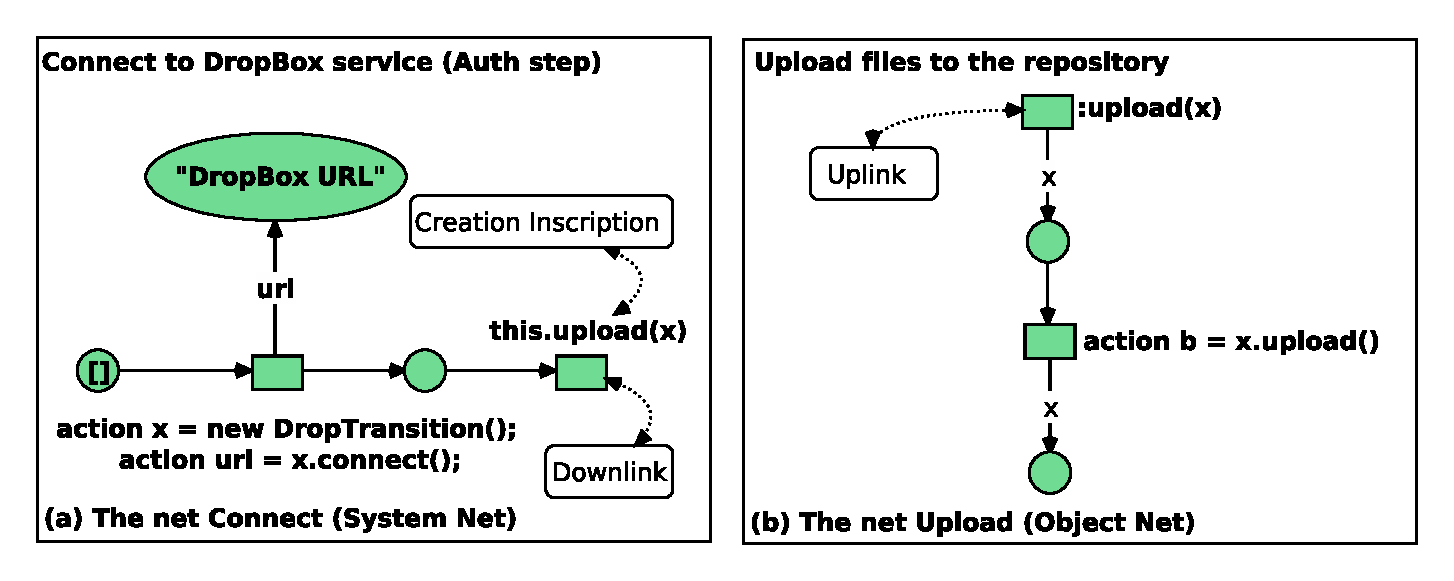
\includegraphics[width=0.79\textwidth,height=0.23\textheight]{images/SystemObjectNet}
\caption{(a) The System Net, (b) The Sub-net Upload}
\label{figure:refnets}
\end{figure}




%Renew 

\subsection{\Renew{}}
%
The \textbf{RE}ference \textbf{NE}ts \textbf{W}orkshop (\Renew{}), which is available at (\url{http://www.renew.de/}) is a graphical tool for creating, editing and simulating reference nets.
%
It combines the \textit{nets-within-nets} paradigm with the implementing power of Java.
%
%
%
With \Renew{} it is possible to draw and simulate both Petri nets and reference nets. 
%
%
%
During the simulation, a net instance is created and can be viewed in a separate window as its active transitions fire.
%
Simulation is used in Renew to view firing sequences of active transitions in reference nets.
%
Simulation can run in a one step modus where users can progress in steps where only one transition fires. 
%
\Renew{} also offers the possibility to set breakpoints to hold the simulation process.
%
Breakpoints can be set to places and transitions. 
%
By changing the compiler, \Renew{} can also simulate P/T nets, timed petri nets, Workflow nets, etc.

\Renew{} is an editor as well as a simulator for Petri nets and \textit{reference nets}.
%%Plug-in system
Since the version 1.7, \Renew{} is built on a highly sophisticated plug-in architecture, which was developed and introduced in \cite{Schleinzer+08}.
%
It allows the extension of \Renew{} with additional functionality through the use of interfaces from \Renew{} components without changing the core of \Renew{}.

%\subsection{Objectives}
%
\subsection{The Grass GIS}
%
\label{subsec:grassgis}
%Here we give an overview of the Grass GIS.
%
Grass is a multi-purpose open source GIS, which can be used for geoprocessing applications such as: geospatial data production, analysis and mapping. 
%
It can handle raster as well vector data.
%
The most important specificity of the Grass GIS is its modularity, which diminishes overhead.
%
This allows to run only the required modules (same as \Renew{}).
%
These modules are organized in categories (general GIS modules, raster modules, vector modules, etc.).
%
Table. \ref{tab:grasscommands} shows the modules provided by the Grass GIS \cite{Neteler+12}.

\begin{table}[!t]
\renewcommand{\arraystretch}{1.3}
\caption{Grass GIS Commands (from \cite{Neteler+12})}
\label{tab:grasscommands}
\centering
\begin{tabular}{c||c||c}
\hline
\bfseries Prefix & \bfseries Function class & \bfseries Type of command\\
\hline\hline
d.* & display & graphical output\\
\hline\hline
db.* & database & database management\\
\hline\hline
g.* & general & general file operations\\
\hline\hline
i.* & imagery & image processing\\
\hline\hline
m.* & misc & miscellaneous commands\\
\hline\hline
ps.* & postscript & map creation in Postscript format\\
\hline\hline
r.* & raster & 2D raster data processing\\
\hline\hline
r3.* & 3D raster & 3D raster data processing\\
\hline\hline
v.* & vector & 2D and 3D vector data processing\\
\hline
\end{tabular}
\end{table}


In order to allow \Renew{} executing these commands directly from the Petri net transitions, \RenewGrass{} offers a wrapping layer, which makes the Grass modules available at runtime.
%
Before using the modules for processing the data, the latter should be first imported into a Grass \textit{DATABASE}.\\
%
Within the DATABASE, the projects are organized as subdirectories called "LOCATIONS".
%
Each LOCATION can have one or more MAPSETS. 
%
Each \textit{MAPSET} may represent a sub region within a given LOCATION.
%
These are mostly the important variables that need to be set.






\section{\RenewGrass{}}
%!TEX root = ./FMi_2015_AISC.tex
%
% UTF8-Check: Umlaute: äöüÄÖÜß
%
\label{sec:grassintegration}
In this section, we show how the Grass GIS has been integrated in \Renew{}.
%
First, a short overview of the Grass GIS is given. 
%
This includes the Grass modules as well as the required structure of a GIS project. 
%
Next, we introduce the architecture to show all the components taking part to the integration.
%
%Somewhere here we must add the literature already published on \RenewGrass{}

\subsection{Integration Issues}
%
The first obstacle we faced when trying to integrate the Grass GIS with \Renew{} is that these tools are written in different programming languages.
(The Grass GIS is written in C and \Renew{} in Java), which makes a direct communication between them arduous.
%
Thus the Grass GIS needs to be adapted to the running environment of \Renew{}.
%
Moreover, a proper environment variables need to be pre-specified.
%
In order to achieve this integration, there are three possibilities:

\begin{itemize}
 \item
 \emph{Desktop integration}: 
 this means that the Grass GIS is locally deployed and interfaces are provided to use geoprocessing functions from \Renew{}.
\item
 \emph{Web-based integration}: 
 in this case, the objective is to publish and execute geo-processes over the web, following the Web Processing Service (WPS) interface specification\footnote{\url{http://www.opengeospatial.org/standards/wps}} from the Open Geospatial Consortium (OGC)\footnote{\url{http://www.opengeospatial.org/}}.
\item
\emph{Remote execution (Vagrant)}: 
this is another alternative to deploy the Grass GIS into the Cloud and is discussed in Section.~\ref{sec:discussion}.

\end{itemize}

%In this paper, we focus on the first solution.
%
%The integration using the WPS is here omitted but we are currently investigating this issue in another work, which concerns the perspective of moving the actual work to be executed in the cloud (see Section.~\ref{sec:discussion}).  
%
Fig.~\ref{fig:overview} is a simple overview of the integration of Grass GIS as desktop application. 
%
With \Renew{} scientific workflows are specified as Petri net models. 
%
When some of workflow tasks require Grass commands, this can be easily performed directly at the transitions.
%
In order to communicate directly with the Grass GIS, an interface or a wrapper is necessary. 

Over the last few years some effort has been dedicated to leverage the strength of Java and Grass GIS. 
%
There are some contributions dealing with this issue \cite{moldt18}. 
%
Two candidate projects are interesting for our work, which are the \textit{JGrasstools}%
\footnote{\url{http://moovida.github.io/jgrasstools/}} 
and the \textit{vtkGRASSBridge}%
\footnote{\url{https://code.google.com/p/vtk-grass-bridge/}}.
%
The \textit{vtkGRASSBridge} provides a VTK/C++ interface to most of the GIS GRASS raster, voxel and vector C library functions
%
This library can be used to build comprehensive 3D visualisation of GIS GRASS data with Java, Python and C++.
%
Although the project seems promising, it was quickly rejected, due to building issues. 
%
We realized, that future users of the tool will certainly run into similar issues, when modeling and executing workflows with \RenewGrass{} if we followed this approach.
%
For this work, we chose to take advantages from the JGrasstools project.
%
JGrasstools is a library that is extracted from the Java Geographic Resources Analysis Support System (JGrass) project.%
\footnote{JGrass is a free, multi platform, open source GIS based on the GIS framework (see \url{www.jgrass.org}).}
%

\begin{figure}[!t]
\centering
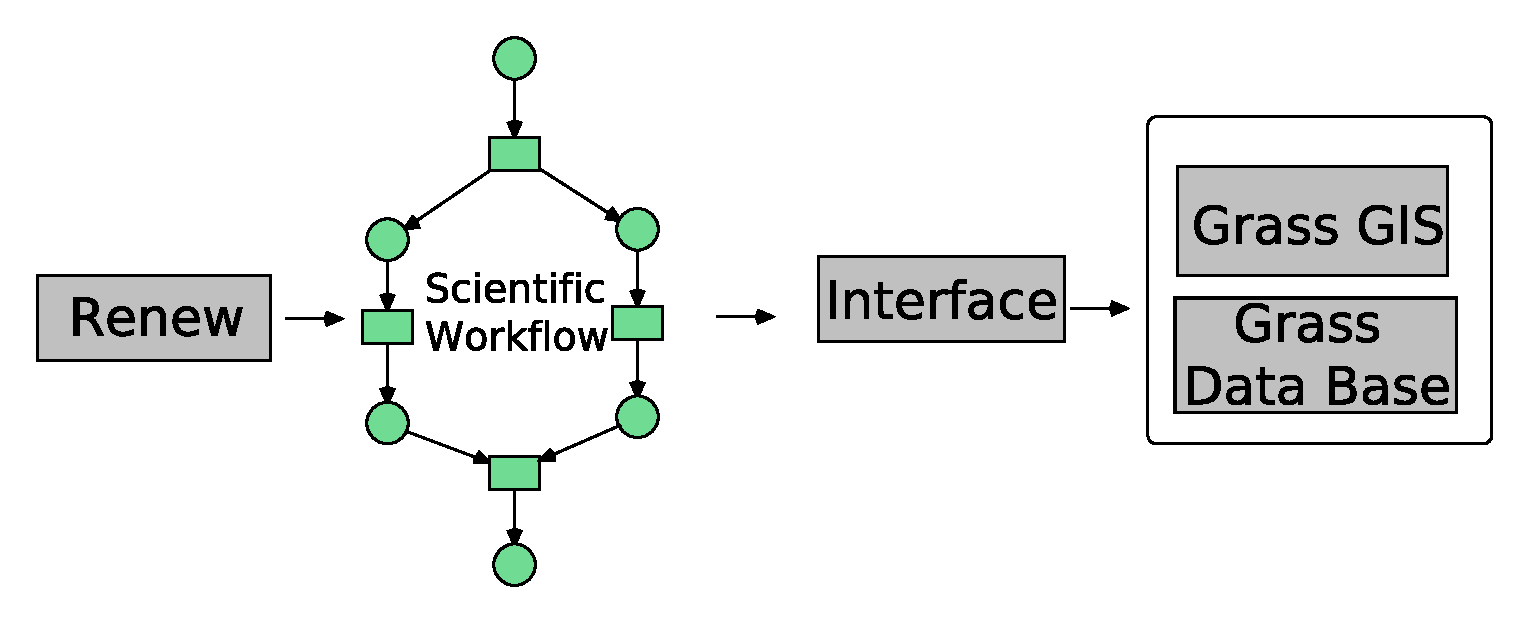
\includegraphics[width=0.78\textwidth,height=0.24\textheight]{images/overview}
\caption{Grass GIS Integration with \Renew{}}
\label{fig:overview}
\end{figure}


\subsection{Architecture}
\label{sec:arch}
%
As mentioned above, \Renew{}'s architecture has been decomposed into several components.
%
Each component is characterized as a plug-in.
%
This provides more flexibility and extensibility.
%
Thus new features can be easily integrated.
%
The basis for this is the \Renew{} plug-in system \cite{Duvigneau10}, which is responsible for the addition and the removal of plug-ins at runtime.


%
New features include some new plug-ins as for instance the \emph{Workflow} and the \emph{WFNet}, which provide workflow management functionality.
%
The original functionality was already presented in \cite{Jacob+02a}.
%
The \RenewGrass{} tool is also built following the plug-in architecture of \Renew{}.
%
Fig.~\ref{fig:renewgrass} shows a simplified view of the position of \RenewGrass{} in \Renew{}.
%

The \emph{Workflow} and the \emph{WFNet} plug-ins are not required when using \RenewGrass{}. 
%
They are used especially when the users want to integrate workflow management functionality such as log-in, tasks management, etc. 
%
As you can see in the figure, the \RenewGrass{} plug-in is built on top of the JGrasstools, which was adapted for \Renew{}.
%
The main requirements are the Grass GIS installation and the Grass data. 
%
The first one provides all the modules presented in Section.~\ref{subsec:grassgis}. 
%
The Grass data is a directory, that holds all the required files (raster or vector images).
%
Both Grass GIS installation and the Grass Data path should be specified to \RenewGrass{} prior any utilization.
%
The actual implementation of the tool allows local execution only, since both \Renew{} and Grass GIS are installed on-premise. 
%
The use of external resources, mainly Cloud computing resources, is not excluded, but it is out of scope of this paper.
%
\RenewGrass{} is freely available via \url{www.paose.net} and \url{http://sofianeb.github.io/}.
%


\begin{figure}[!t]
\centering
%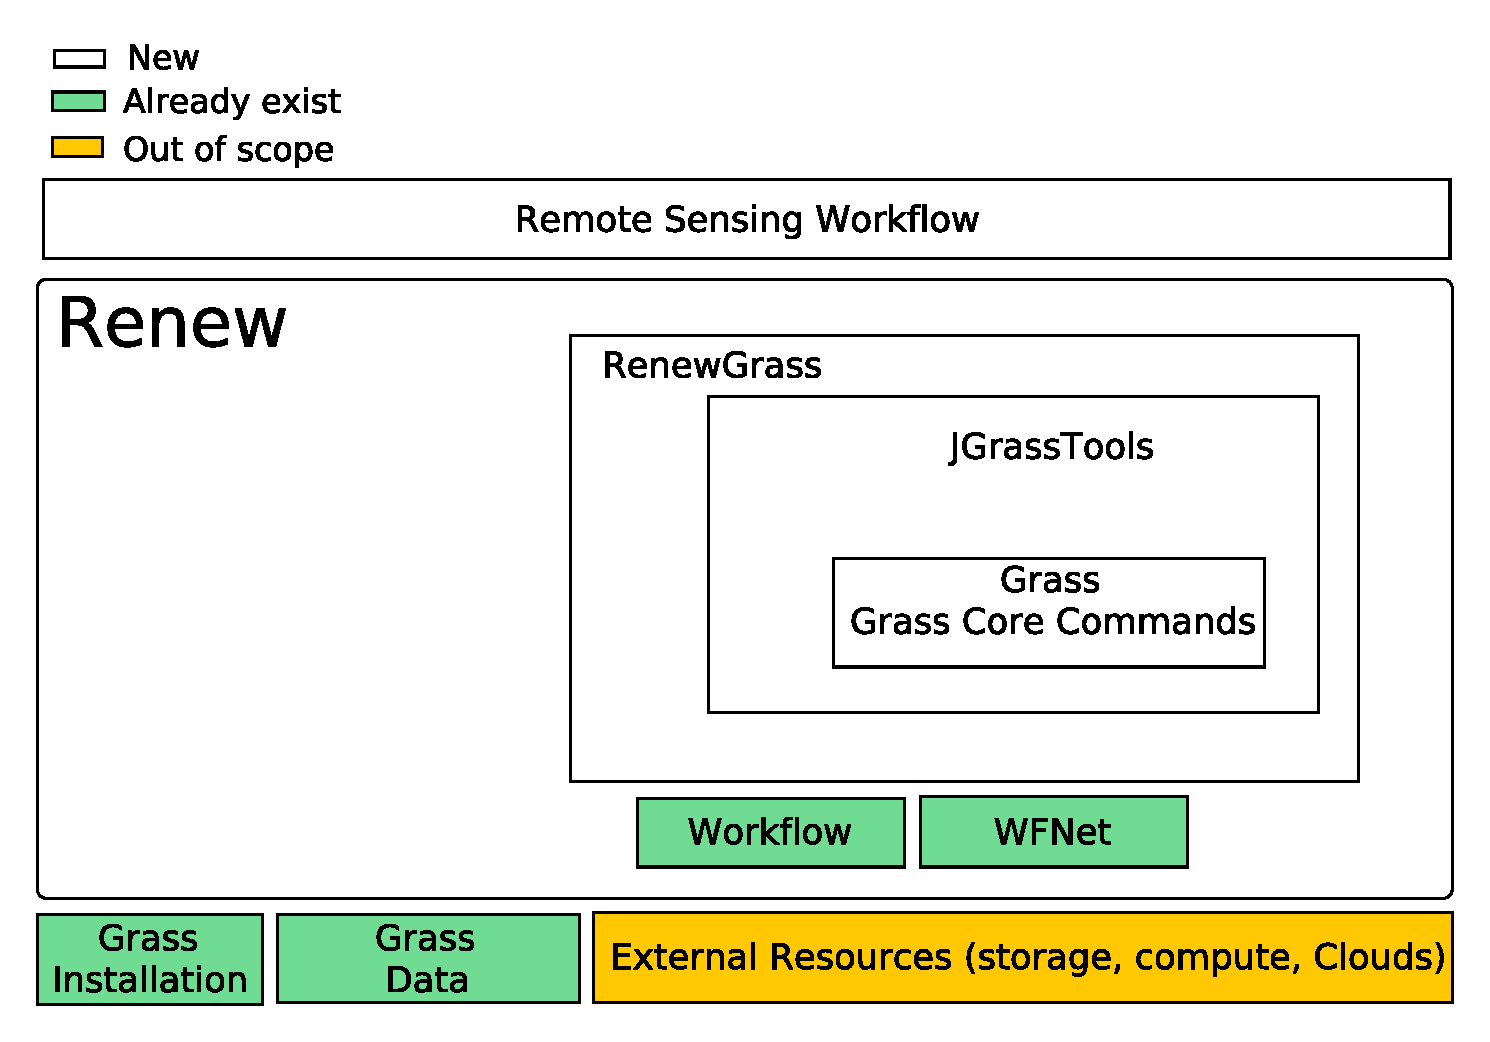
\includegraphics[width=0.78\textwidth,height=0.30\textheight]{images/ArchitectureGrassRenew2}
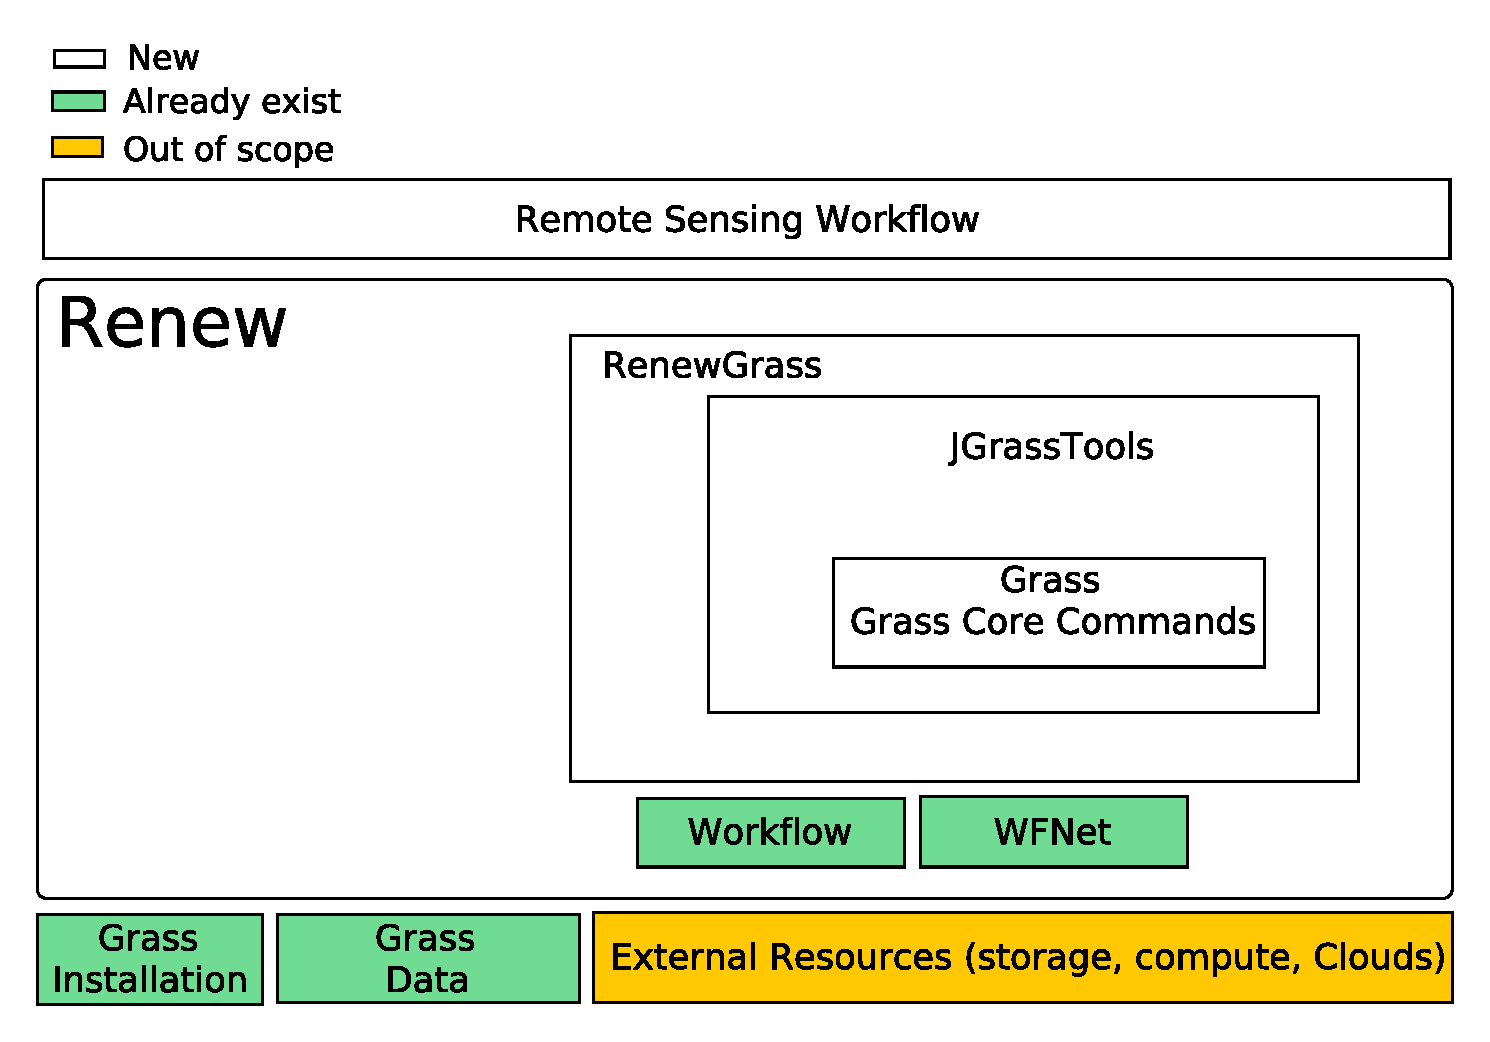
\includegraphics[width=\textwidth]{images/ArchitectureGrassRenew2}
\caption{Architecture of the \RenewGrass{} Tool}
\label{fig:renewgrass}
\end{figure}
%EOF





\section{\RenewGrass{} in the Cloud}
\label{sec:Cloudmigration}
%
\RenewGrass{} has been successfully tested in a local environment.
%
All the required components were hosted on-premise (\Renew{}, Grass GIS and the data).
%
Nevertheless, as soon as the number of tasks increases and the size of data become large, we start facing computing and storage issues.
%
This is due to insufficient resources on the local site.
%
This section presents our vision to deploy the current implementation of the \RenewGrass{} tool onto the Cloud services.
%
First, different possibilities to Cloud-enable an application in general are shortly illustrated.
%
These possibilities are formulated in form of patterns.
%
The illustration is based on the work of \cite{han10} and \cite{leyman09}.
%
They investigate and strive to answer questions like: where to enact the processes? Where to execute the activities? and Where to store the data?
%
Thus the entities taken in account are: (1) the process engine (responsible for the execution and the monitoring of the activities) (2) the activities that need to be executed by the workflow and (3) the Data.
%
Next, we propose an architecture to introduce a new pattern and an appropriate methodology to enable remote execution in the Cloud.
%
This has been also described in a previous work \cite{Bendoukha+15}.
%
\subsection{Migration Patterns}
%
Moving an existing application to the Cloud should be based on a solid strategy.
%
Providing the business management system (or WfMS) or a part in the Cloud raises a series of concerns about ensuring the security of the data and the performance of the system. 
%
For example, Cloud users could lose control on their own data in case of a fully Cloud-based solution. 
%
Some activities, which are not compute-intensive can be executed on-premise rather than moving them to the Cloud. 
%
Unfortunately, this transfer can be time and cost-consuming because of the pay-per-use model and the nature of the workflow tasks.


%
%
%
%
In the following, the patterns from \cite{han10,leyman09} are shortly introduced.
%
%
%
The first pattern designs the traditional scenario where all the components of the workflow system are hosted at the user-side (on-premise).
%
The second scenario represents a case when users already have a workflow engine but the application contains compute or data-intensive activities, so they are moved to the Cloud for acquiring more capabilities and better performance.
%
The third case designs a situation, where the end-users do not have a workflow engine, so they use a Cloud-based workflow engine, which is provided on-demand.
%
In that case, workflow designers can specify transfer requirements of activity execution and data storage, for example, sensitive data and non-compute-intensive activities can be hosted on-premise, and compute-intensive activities and non-sensitive data can be moved to the Cloud \cite{han10}.
%
%
The last scenario presents a situation where all components are hosted in a Cloud and accessed probably from a Web interface.
%
The advantage is that users do not need to install and configure any software on the user side.
%
%
%
%
%
To make an analogy with the elements of our approach, \Renew{} is the process engine, the activities are the geoprocessing tasks (performed by the Grass services), which are related to the satellite images (data).
%
The latter (data and Grass GIS) can be either on-premise or hosted in the Cloud.
%
Based on these elements and the illustration presented above, Fig.~\ref{fig:cloudpatterns} presents an overview of the diverse approaches (patterns) to design our workflow system based on the Cloud technology.
%
\begin{figure}[!t]
    \centering
 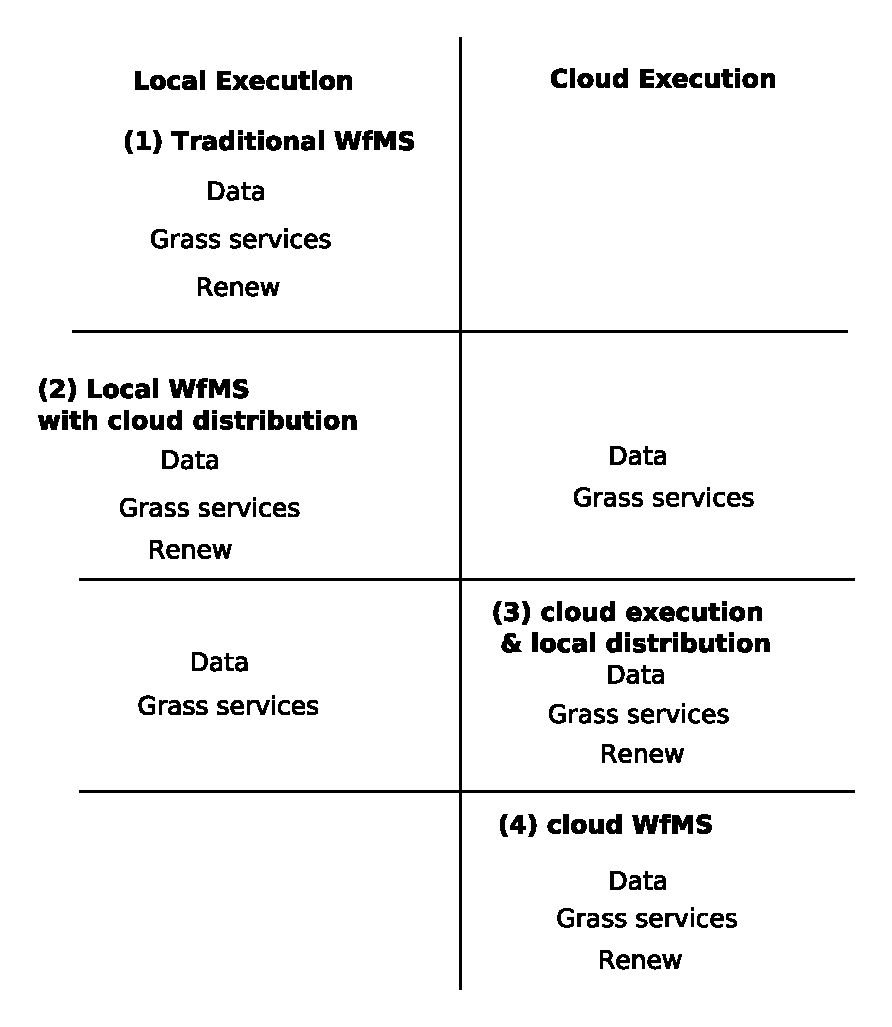
\includegraphics[width=0.68\textwidth,height=0.35\textheight]{images/CloudGrassPatterns}
\caption{Patterns for Cloud-based Workflow Systems (Adapted from \cite{han10})}
\label{fig:cloudpatterns}
\end{figure}



%%%%our work

We have noticed that both \cite{han10} and \cite{leyman09} do not address all possible situations.
%
For instance, the following situation has been not addressed: the process engine is available on the user side but due to circumstances (internal failure, not sufficient compute or storage resources), remote process engines need to be integrated and remotely invoked.
%
Fig. \ref{fig:pattern5} shows approximately how this scenario looks like.
%
Our solution consists on transferring the data and executing the process by another process engine.
%
This is discussed in the following sections. 
%
% 
%
%
\begin{figure}[!t]
    \centering
  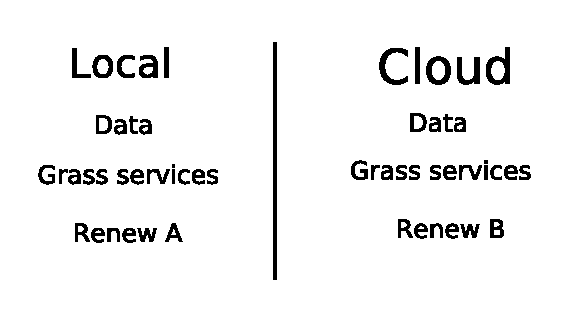
\includegraphics[width=0.48\textwidth,height=0.10\textheight]{images/pattern5}
\caption{A Pattern Designing Multiple Process Engines Integration}
\label{fig:pattern5}
\end{figure}

\subsection{Architecture}
%
Fig. \ref{fig:architecture} shows the architecture to integrate the current implementation into a Cloud system.
%
While \RenewGrass{} is already implemented and successfully integrated in \Renew{} (see section \ref{sec:grassintegration}), most efforts are dedicated now to move the execution of the geoprocessing tasks to the Cloud and the provision of an interface to invoke these services  directly from workflow models.

In our work, we follow an agent-based approach, i.e., many components functionalities are performed by special agents.
%
In summary, the role of each agent used in the approach is described below.
%
\begin{enumerate}
 \item 
 \textit{Workflow Holder Agent}:
 %
 The Workflow holder is the entity that specifies the workflow and in consequence holds the generated Petri net models.
 %
 This entity can be either human or a software component.
 %
 The specification of the image processing workflow is performed using \RenewGrass{}, which provides a modeling palette or downright predefined modeling blocks.
\item 
 \textit{Cloud Portal Agent}:
 %
 provides the \textit{Workflow Holder Agent} a Web portal as a primary interface to the whole system.
 %
 It contains two components: \textit{Cloud Manager} and \textit{Workflow Submission Interface}.
 %
 The latter provides a Web interface to the workflow holders to upload all necessary files to execute the workflow.
 %
 This includes the workflow specification (\Renew{} formats\footnote{\Renew{} supports various file formats saving (XML, .rnw, .sns, etc.)}), input files (images).
 %
 It also serves getting notifications from the \textit{Cloud Broker Agent} about the status of the workflow or the availability of the Cloud provider.
%
The role of the \textit{Cloud Manager} is to control the Cloud instances (start and stop or suspend).

 % 
% 
%
% 
 \item 
 \textit{Cloud Broker Agent}:
 %
 It is a critical component of the architecture, since it is responsible of (i) the evaluation and selection of the Cloud providers that fits the workflow's requirements (e.g., data volume and computing intensities) and (ii) mapping the workflow tasks.% to that Cloud provider to be executed. 
 %
 Both activities require information about the Cloud provider, which are available and provided by the Cloud Repository Agent.
 \item 
 \textit{Cloud Repository Agent}:
 The Cloud repository register the information about the Cloud providers and the state of their services.
 %
 These information are saved in a database and are constantly updated, since they are required by the Cloud Broker Agent.
 %
 To avoid failure scenarios (repository down, loss of data), we use distributed databases, which allows high availability and fault-tolerant persistence.
\item 
 \textit{Cloud Provider Agent}:
The role of this agent is to control the instances and to manage the execution of the tasks.
%
Regularly, the Cloud providers need to update their status and send it to the Cloud Repository Agent.
%
The status concerns both the instance and the services (Grass services).
\end{enumerate}


\begin{figure*}[!t]
    \centering
  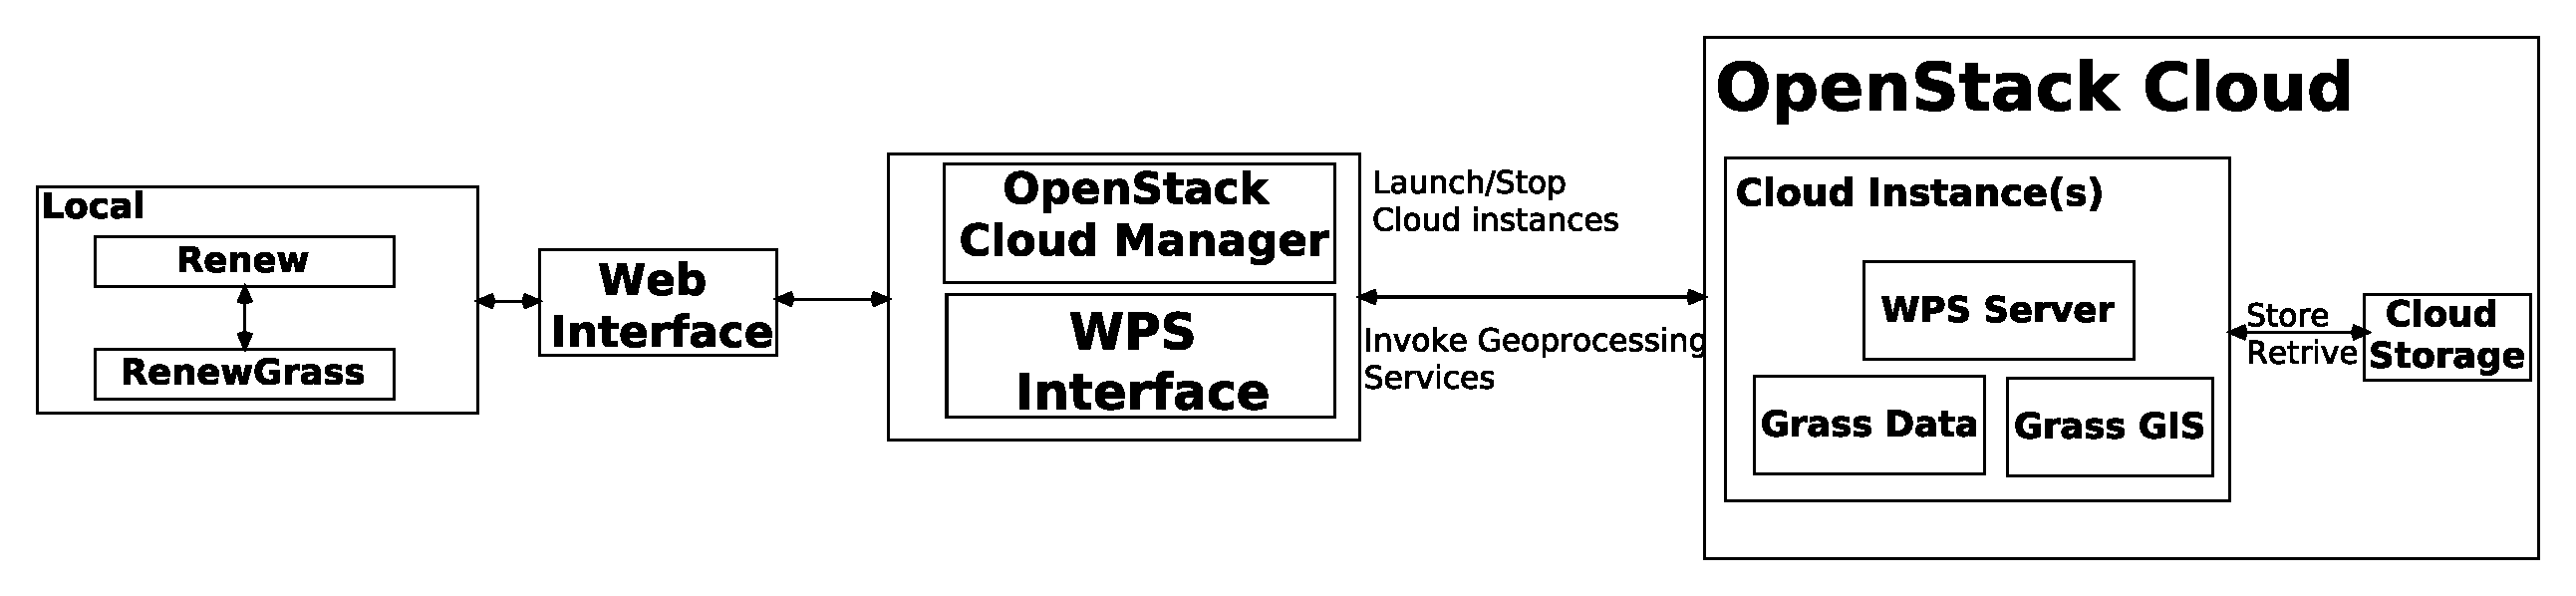
\includegraphics[width=0.98\textwidth,height=0.20\textheight]{images/GrassMigration}
\caption{The Architecture of the Cloud-based Workflow System}
\label{fig:architecture}
\end{figure*}



%%%%%
Concerning the \textit{Cloud Broker Agent}, the evaluation and the selection of the Cloud providers are critical processes for the \textit{Workflow Holders}.
%
In Cloud computing there are various factors impacting the Cloud provider evaluation and selection \cite{Haddad11,Badger+11a} such as: computational capacity, IT security and privacy, reliability and trustworthiness, customization degree and flexibility/scalability, manageability/usability and customer service, geolocations of Cloud infrastructures. 
%
For this, in our work, brokering factors are limited to the computational capacity and the customization degree. 

%
\subsection{Cloud Configuration}
%
Concerning the customization degree, there are some requirements for a successful deployment onto the Cloud.
%
In general, a common procedure to deploy applications onto Cloud services consists of these two main steps: 
%
\begin{enumerate}
 \item 
 \textit{set up the environment}: 
 %
 this mainly consists of the provision of Cloud instances\footnote{The Cloud instances should be in priori customized, i.e, they need to have the Grass GIS as back-end, the WPS server and \Renew{}.
 %
 We assume that the Cloud storage is a service, which is configured by the Cloud provider itself.
 } and the configuration the required softwares properly.
 %
 %
 Essential are the environment variables, which differ from the local implementation such as JAVA configuration for the Web server.
 %
 \item
 \textit{deploy the application}: it consists of the customization of the Cloud instance with the appropriate softwares. 
 %
 For our work, \Renew{} and the Grass GIS should be correctly and properly configured, especially the database and the installation path.
 
 \end{enumerate}
 

%
Furthermore, the Grass commands can be invoked in different ways. 
%
Either through a wrapper like in the original implementation of \RenewGrass{} or provided as Web services.
%
For the latter, we follow a Web-based approach with respect to the Open Geospatial Consortium (OGC) Web Processing Service (WPS) interface specification. 
%
Thus the Grass GIS functionalities are provided as Web services instead of desktop application.
%
To achieve this, we chose the 52North\footnote{http://52north.org/} as a WPS server as well as the wps-grass-bridge\footnote{https://code.google.com/p/wps-grass-bridge/}.

%
\subsection{Execution Scenario}

Considering the proposed architecture and the agent roles described above, a typical deployment scenario is broken into the following steps: 
%
\begin{enumerate}
 \item 
Workflow holders specify their image processing workflows (data and control-flow) using Petri nets for example the NDVI workflow (see section \ref{sec:grassintegration}).
\item 
They send a request to the \textit{Cloud Broker} via the \textit{Cloud Portal}.  
\item
The \textit{Cloud Broker} checks for available Cloud providers, which provide geoprocessing tools (Grass GIS).
%
This information is retrieved from the \textit{Cloud Repository}.
%
\item
The \textit{Cloud Broker} sends a list to the \textit{Workflow Holder} (through the Cloud Portal) to accept or to reject the offer.
\item
If the offer is accepted, the \textit{Workflow Holder} submits the workflow specification (.rnw + .sns) to the selected \textit{Cloud Provider}.
\item
Launch a customized Cloud instance with \Renew{} and Grass GIS running in the background.
\item 
After simulation/execution of the workflow, results (in our prototype it consists of calculating the NDVI value) are transmitted to the \textit{Workflow Holder} through the \textit{Cloud Portal}.
\end{enumerate}

Rejecting an offer does not conclude the execution process immediately. 
%
Since the list transmitted by the \textit{Cloud Broker} is updated constantly,
%
it might be that new Cloud providers are available and fits the requirements.
%
Therefore, from step (3), the process is iterative until the satisfaction of the \textit{Workflow Holder}.
%
Regarding step (5) and (6), \Renew{} supports starting a simulation from the command line.
%
This is possible by using the command \textit{startsimulation (net system) (primary net) [-i]}.
%
The parameters to this command have the following meaning:
%
\begin{itemize}
 \item 
 \textit{net system}: The .sns file.
\item 
 \textit{primary net}: The name of the net, of which a net instance shall be opened when the simulation starts. 
\item
-i: If you set this optional flag, then the simulation is initialized only, that is, the primary
net instance is opened, but the simulation is not started automatically.
\end{itemize}

%In a future paper, we will give a first evaluation of the presented work as well as the progress of the implementation of the components presented in this section.
%
%Furthermore, we have implemented other image processing workflows such as the Normalized Differences Vegetation Index (NDVI). 


\section{Discussion}
\label{sec:discussion}
%
In the previous sections we presented \RenewGrass{} and its integration in the modeling and simulation tool \Renew{}. 
%
We explained that there are many possibilities to deploy the tool. 
%
Either on-premise or in the Cloud.
%
For now \RenewGrass{} has been successfully deployed in local environment following \emph{Desktop integration} (see Section.~\ref{sec:grassintegration}). 
%
Grass GIS modules can be easily invoked from Petri net models.
%
Concerning the deployment of \RenewGrass{} into the Cloud, the proposed solution involves the provision of Grass functionalities as Web services using the WPS specification (see Section.~\ref{sec:Cloudmigration}). 
%
Here we discuss another alternative to deploy \RenewGrass{} into the Cloud.
%
Our solution consists of creating customized Cloud instances, which includes \Renew{} and the Grass GIS.
%
Thus all activities are performed in the Cloud.
%
The idea is that Cloud customers have the possibility to specify image processing workflows using Petri nets.
%
The latter are then pushed to the Cloud, where they are executed/simulated.
%
This scenario is summarized in Fig.~\ref{fig:renew_cloud}.
%
Our concept is based on enabling \Renew{} simulations in the Cloud.
%
We already provide mechanisms to Cloud customers to create Cloud instances and provision them by Java, \Renew{} and other softwares that they need for running their applications \cite{Bendoukha+15a}.
%

\begin{figure}[!t]
\centering
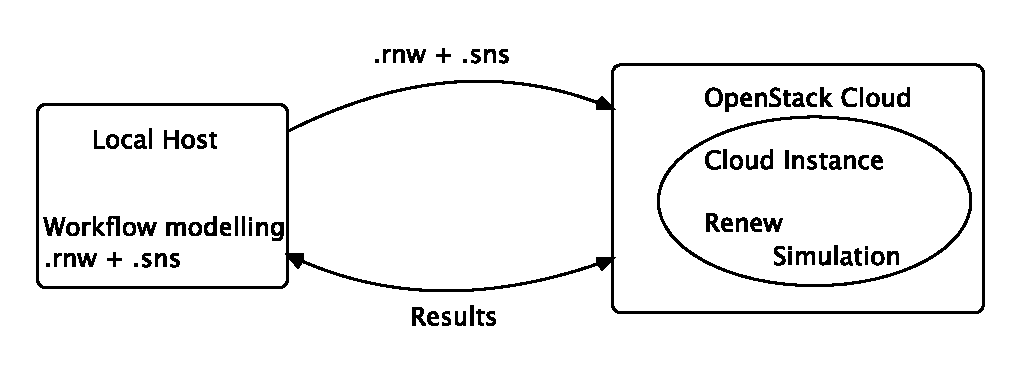
\includegraphics[width=0.7\textwidth]{images/openstacksimulation}
\caption{\Renew{} Simulation in the Cloud (from \cite{Bendoukha+15a})}
\label{fig:renew_cloud}
\end{figure}
%
 
Unfortunately, the current solution raises other interesting issues that need more investigation.
%
For example,  our proposition is based on the fact that workflows are executed once as a single process.
%
There is at the moment no mechanism to control the simulation of the workflow in the Cloud.
%
We mean by \emph{control}: the management of firing the Petri nets transitions in the Cloud instance. 
%
\Renew{} already provides the possibility to control the simulation by specific commands like: \emph{simulation run}, \emph{simulation halt} or \emph{simulation stop}.
%\footnote{More information about these commands can be found in \cite[p.106]{Kummer+13a}.}.  
%
Nevertheless, it is not possible to use these functionalities within a Cloud instance.
%
This should be in priori customized.
%
What about the ability to decompose the workflow in order enable selected execution of the tasks composing the workflow?
%
For this purpose we are investigating other alternatives as the remote execution of \Renew{}.
%
One of these solutions have been already discussed in \cite{Bendoukha+15a}.
%
In the latter work we provide mechanisms and implementation for moving the execution of computation- and time- consuming workflows into the Cloud.
%
Different kind of interfaces are provided to enable remote execution of \Renew{} in the Cloud.
%
These interfaces define how input and output to the Cloud calls are defined.
%
They range from simple, simulation and complex.

Interesting for the current work are the complex interfaces.
%
Through such kind of interface we seek bringing intelligence and autonomy to the managing system.
%
Concretely, special \emph{agents} are used as \emph{gateways} between the workflow (Petri net) model and the Cloud.
%
With respect to the \Mulan{}/\Capa{} framework, there exists a \emph{WebGateway Agent} \cite{Betz+14}.
%
It plays the role of a gateway between \Renew{} and the Web environment. 
%
Since Grass GIS commands can be also published as Web services (see Section.~\ref{sec:Cloudmigration}) coupling the WebGateway functionality into the architecture proposed in Section.~\ref{sec:Cloudmigration} will certainly enhance building agent-based scientific workflows.




\section{Conclusion}
\label{sec:conclusion}
%
The objective of the work presented in this paper is twofold.
%
On the one side, we provide techniques and tools to support scientists building their applications.
%
For this purpose, a geoprocessing tool named \RenewGrass{} is presented.
%
The tool has been implemented and successfully integrated in the modeling and simulation tool \Renew{}.
%the implementation of a geoprocessing tool  for \Renew{}.  
%
%This tool extends \Renew{} to be able to support another kind of workflows (scientific workflows) apart the business workflows. 
%
The application domain of \RenewGrass{} is the remote sensing, especially image processing, a kind of scientific workflows. 
%
Therefore, we afford scientists with a palette of processing functionalities based on the Grass GIS. 
%
Furthermore, we discuss the extension of the current work by the integration of the Cloud technology. 
%
%Although the first objectives are reached, we are actively working to enable the \RenewGrass{} in the Cloud.
For this purpose, we introduce migration patterns and introduced our architecture for the deployment of workflows onto Cloud providers. 
%
The natural next step is to concertize the deployment mechanisms introduced in Section~\ref{sec:Cloudmigration}.
%
This means concretely to implement the functionality of each agent.
%
In our perspective, this can be performed by using the \Mulan{}/\Capa{} framework and following the \Paose{} approach.





\bibliography{FMi_2015_AISC}

\bibliographystyle{plain}
\end{document}
